\documentclass[tikz,border=10pt]{standalone}
\usepackage{tikz}
\begin{document}
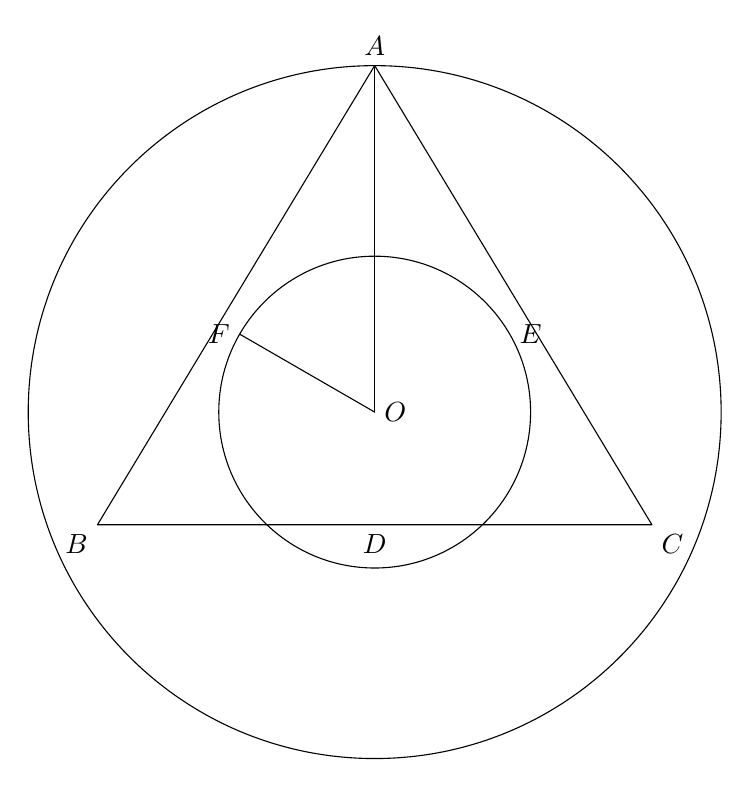
\begin{tikzpicture}[scale=1.1, line cap=round, line join=round]

% Key points
\coordinate (O) at (0,0);
\coordinate (A) at (0,4);
\coordinate (B) at (-3.2,-1.3);
\coordinate (C) at (3.2,-1.3);
\coordinate (D) at (0,-1.3);

% Inner circle radius
\def\r{1.8}

% Tangency points on the inner circle
\coordinate (F) at ({-\r*0.8660254},{\r*0.5});
\coordinate (E) at ({ \r*0.8660254},{\r*0.5});

% Outer circle radius
\def\R{4}

% Circles
\draw (O) circle (\R);
\draw (O) circle (\r);

% Triangle
\draw (A)--(B)--(C)--cycle;

% Radius / diameter-like segment
\draw (A)--(O);

% Extra segment
\draw (O)--(F);

% Labels
\node[above] at (A) {$A$};
\node[below left] at (B) {$B$};
\node[below right] at (C) {$C$};
\node[below] at (D) {$D$};
\node[right] at (O) {$O$};
\node[left] at (F) {$F$};
\node[right] at (E) {$E$};

\end{tikzpicture}
\end{document}
